% ================= 1. KHẢO SÁT =================
\section{Khảo sát}

\begin{frame}{Bước khảo sát cho ra 4 output}
\centering
\begin{tikzpicture}[hd/.style={font=\small\bfseries, text=white}]
\node[obox=tvA!8] (o1) at (0,0) {};
\node[obox=tvA!8] (o2) at (3.75,0) {};
\node[obox=tvB!8] (o3) at (7.5,0) {};
\node[obox=tvB!8] (o4) at (11.25,0) {};
\foreach \n/\t/\c in {o1/{Output 1}/tvA, o2/{Output 2}/tvA, o3/{Output 3}/tvB, o4/{Output 4}/tvB}{
  \node[fill=\c, rounded corners=2pt, minimum width=3.3cm, hd] at (\n.north) {\t};}
\node[text width=3.1cm, font=\scriptsize, align=left, below=4mm of o1.north] {\textbf{Mô tả bài toán \& hiện trạng theo 4W+1H}\\[2pt]
  What -- Who -- Where -- When -- How; tác nhân, bộ phận, điểm yếu của cách làm hiện tại $\Rightarrow$ phạm vi hệ thống.};
\node[text width=3.1cm, font=\scriptsize, align=left, below=4mm of o2.north] {\textbf{Hồ sơ biểu mẫu thu thập}\\[2pt]
  5 biểu mẫu nghiệp vụ (phiếu yêu cầu, phiếu theo dõi xử lý, hồ sơ khách, phiếu đặt phòng, phiếu khảo sát) $\Rightarrow$ trường dữ liệu, cột lưới, ô nhập.};
\node[text width=3.1cm, font=\scriptsize, align=left, below=4mm of o3.north] {\textbf{Danh sách yêu cầu}\\[2pt]
  Yêu cầu chức năng $\Rightarrow$ \textbf{10 Use Case} theo tác nhân; yêu cầu phi chức năng (bảo mật, cấu hình, đóng gói, ngôn ngữ).};
\node[text width=3.1cm, font=\scriptsize, align=left, below=4mm of o4.north] {\textbf{Quy tắc nghiệp vụ \& từ điển số liệu}\\[2pt]
  \textbf{11 quy tắc} (TV1: 1--5, TV2: 6--10, chung: 11) và các con số: SLA, hệ số ưu tiên, hạng thành viên, ngưỡng điểm.};
\draw[-{Stealth},thick,navy] (o1.east) -- (o2.west);
\draw[-{Stealth},thick,navy] (o2.east) -- (o3.west);
\draw[-{Stealth},thick,navy] (o3.east) -- (o4.west);
\node[draw=navy, fill=navy!8, rounded corners=3pt, font=\scriptsize, text width=14.6cm, align=center] at (5.62,-2.65)
  {Đầu vào cho bước \textbf{Phân tích}: Output 1+3 $\to$ \textbf{BFD} \quad|\quad Output 2+4 $\to$ \textbf{sơ đồ thực thể liên kết / biểu đồ lớp} \quad|\quad Output 2 $\to$ \textbf{thiết kế giao diện}};
\end{tikzpicture}

\vspace{1mm}
{\tiny\color{common} Nguồn: đặc tả dự án \code{docs/PLAN.md} (đề CRM áp dụng cho khách sạn). Nội dung hiện trạng là kịch bản khảo sát của nhóm; số liệu nghiệp vụ trùng với hằng số trong code.}
\end{frame}

% ---------- Output 1 ----------
\begin{frame}{Output 1 -- Mô tả bài toán \& hiện trạng theo 4W+1H}
\scriptsize
\begin{tabularx}{\textwidth}{@{}L{1.75cm}Y@{}}
\toprule
\textbf{Câu hỏi} & \textbf{Kết quả khảo sát} \\
\midrule
\textbf{What}\newline Bài toán gì? & Chăm sóc khách lưu trú: \textbf{tiếp nhận -- điều phối -- xử lý -- đóng} các yêu cầu/khiếu nại (ticket) có hạn xử lý (SLA); quản lý hồ sơ khách, đặt phòng/nhận--trả phòng, tích điểm \& hạng thành viên, khảo sát hài lòng, báo cáo hiệu suất. \\
\textbf{Who}\newline Ai tham gia? & \textbf{Manager} (Front Office): phân công, đóng/mở lại ticket, xem báo cáo. \textbf{Agent} (Guest Relations, Housekeeping, Engineering): tạo và xử lý ticket, ghi khảo sát. \textbf{Khách lưu trú}: người được phục vụ, không đăng nhập hệ thống. \\
\textbf{Where}\newline Ở đâu? & Quầy lễ tân và 4 bộ phận: \code{GUEST}, \code{HOUSE}, \code{ENG}, \code{FRONT}. Phần mềm desktop nội bộ, một file chạy, dữ liệu đặt cạnh file chạy. \\
\textbf{When}\newline Khi nào? & Khi khách gọi/đến quầy/email báo sự cố $\to$ lập ticket ngay, hạn tính theo giờ; lúc check-in/check-out $\to$ ghi lịch sử, cộng điểm; ticket đã giải quyết $\to$ khảo sát 1 lần; cuối kỳ $\to$ báo cáo. \\
\textbf{How}\newline Làm thế nào? & \textbf{Hiện trạng:} ghi sổ/Excel, giao việc qua điện thoại, không biết Agent nào đang quá tải, khách VIP không được ưu tiên, không tra được lịch sử khách. \newline
\textbf{Giải pháp:} ứng dụng WinForms 3 tầng; ticket có vòng đời rõ ràng (State); phân công tự động theo tải/bộ phận (Strategy); hạn SLA tính theo loại ticket, mức ưu tiên và hạng khách; tự cộng điểm, tự nâng hạng. \\
\bottomrule
\end{tabularx}
\end{frame}

% ---------- Output 2 ----------
\begin{frame}{Output 2 -- Hồ sơ biểu mẫu thu thập và nơi xuất hiện trong hệ thống}
\scriptsize
\begin{tabularx}{\textwidth}{@{}L{2.55cm}YL{2.55cm}L{3.1cm}@{}}
\toprule
\textbf{Biểu mẫu} & \textbf{Trường dữ liệu chính} & \textbf{Form} & \textbf{Lớp / thuộc tính} \\
\midrule
\textcolor{tvA}{\textbf{BM1}} Phiếu yêu cầu / khiếu nại & Khách, loại yêu cầu, mức độ, tiêu đề, mô tả, phòng (nếu sửa chữa), thời điểm nhận & \code{TicketEditForm} & \code{SupportTicket} (\code{Title}, \code{Priority}, \code{CreatedAt}), \code{MaintenanceTicket.RoomId} \\
\textcolor{tvA}{\textbf{BM2}} Phiếu theo dõi xử lý & Người nhận, trạng thái, hạn xử lý, ghi chú giải quyết, ngày giải quyết/đóng & \code{TicketDetailForm}, \code{TicketListForm} & \code{State}, \code{AssignedAgent}, \code{DueAt}, \code{ResolutionNote}, \code{ClosedAt} \\
\textcolor{tvB}{\textbf{BM3}} Hồ sơ khách / thẻ thành viên & Họ tên, SĐT, email, CCCD/hộ chiếu, quốc tịch, ghi chú, hạng, điểm & \code{CustomerEditForm}, \code{CustomerListForm} & \code{Customer} (\code{IdentityNumber}, \code{Tier}, \code{Points}) \\
\textcolor{tvB}{\textbf{BM4}} Phiếu đặt phòng / nhận--trả phòng & Khách, phòng, loại phòng, giá/đêm, ngày nhận, ngày trả, số đêm, thành tiền, trạng thái & \code{BookingForm} & \code{Booking}, \code{Room}, \code{RoomType} (\code{Nights}, \code{TotalAmount}) \\
\textcolor{tvB}{\textbf{BM5}} Phiếu khảo sát hài lòng & Ticket, điểm 1--5, nhận xét, thời điểm & \code{SurveyForm} (GĐ 4) & \code{SatisfactionSurvey} \\
\bottomrule
\end{tabularx}

\vspace{2mm}
\begin{block}{Truy vết ngược Form $\to$ biểu mẫu (ví dụ)}
Cột \textbf{Total (USD)} trong lưới của \code{BookingForm} lấy từ ô ``thành tiền'' của BM4 = số đêm $\times$ \code{RoomType.PricePerNight}; cột \textbf{Due} trong \code{TicketListForm} là ô ``hạn xử lý'' của BM2, tính bằng \code{SupportTicket.CalculateDueAt()}.
\end{block}
\end{frame}

\begin{frame}{Output 2 -- Ví dụ: Phiếu yêu cầu (BM1) $\leftrightarrow$ màn hình \code{TicketEditForm}}
\begin{columns}[c]
\column{0.46\textwidth}
\centering
\begin{tikzpicture}[font=\scriptsize]
\node[draw=black!60, fill=yellow!6, minimum width=6.2cm, minimum height=5.45cm, drop shadow] (p) {};
\node[anchor=north, font=\small\bfseries] at ($(p.north)+(0,-0.15)$) {PHIẾU YÊU CẦU / KHIẾU NẠI};
\node[anchor=north, font=\tiny] at ($(p.north)+(0,-0.6)$) {Khách sạn ......  -- Số phiếu: ......  -- Giờ nhận: ...h... ngày ../../....};
\foreach \y/\t in {1.3/{Khách hàng (tên, SĐT): ..................................},
                   1.85/{Loại: $\square$ Khiếu nại \ $\square$ Yêu cầu dịch vụ \ $\square$ Sửa chữa},
                   2.4/{Mức độ: $\square$ Thấp \ $\square$ Trung bình \ $\square$ Cao \ $\square$ Khẩn},
                   2.95/{Tiêu đề: ..................................................},
                   3.5/{Nội dung: .................................................},
                   3.95/{\phantom{Nội dung: }.................................................},
                   4.5/{Phòng (nếu sửa chữa): ..........},
                   4.95/{Người tiếp nhận: ............ \quad Ký tên: ............}}
  {\node[anchor=west] at ($(p.north west)+(0.2,-\y)$) {\t};}
\end{tikzpicture}
\column{0.52\textwidth}
\centering
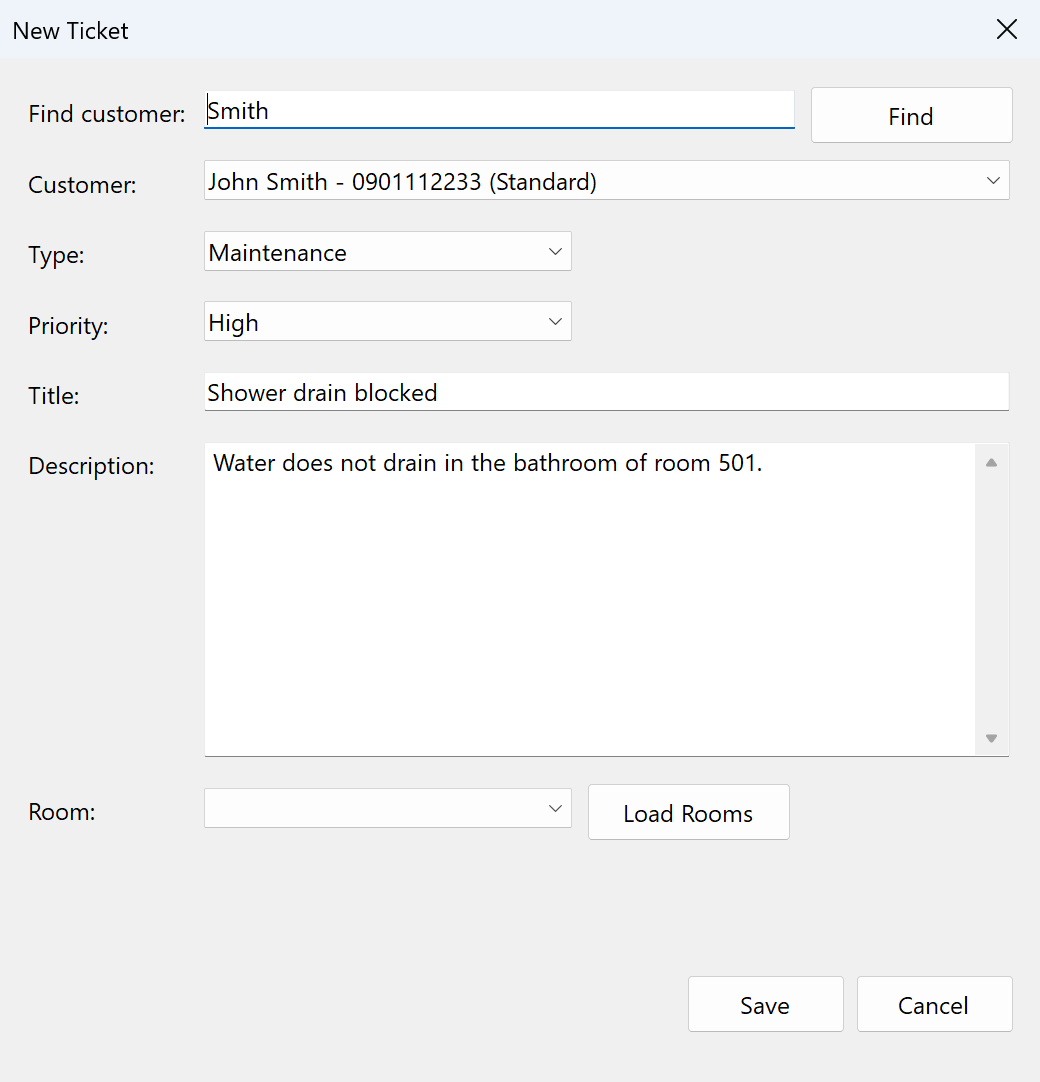
\includegraphics[height=0.66\textheight]{img/04-ticket-edit.png}
\end{columns}
\vspace{1mm}
{\scriptsize Mỗi ô của phiếu thành một control: khách $\to$ \code{txtCustomerKeyword}+\code{cboCustomer}; loại $\to$ \code{cboType} (3 lớp con ticket); mức độ $\to$ \code{cboPriority} (\code{TicketPriority}); phòng $\to$ \code{cboRoom} (chỉ phòng khách đang ở, qua \code{IStayLookup}). Giờ nhận = \code{CreatedAt}, không nhập tay.\par}
\end{frame}

% ---------- Output 3 ----------
\begin{frame}{Output 3 -- Danh sách yêu cầu chức năng $\to$ 10 Use Case}
\begin{columns}[T]
\column{0.62\textwidth}
\scriptsize
\begin{tabularx}{\linewidth}{@{}L{0.55cm}YL{1.55cm}L{0.75cm}L{0.65cm}@{}}
\toprule
\textbf{UC} & \textbf{Yêu cầu chức năng} & \textbf{Tác nhân} & \textbf{TV} & \textbf{Liên PH} \\
\midrule
UC1 & Đăng nhập / đăng xuất & M, A & \TC & \\
UC2 & Tạo ticket (3 loại, tính hạn SLA) & M, A & \TA & \checkmark \\
UC3 & Phân công ticket (tự động / thủ công) & M & \TA & \checkmark \\
UC4 & Xử lý ticket (Start, Resolve, Close, Reopen) & A; M & \TA & \\
UC5 & Tìm kiếm ticket đa tiêu chí & M, A & \TA & \\
UC6 & Quản lý khách hàng (thêm, sửa, xóa, tìm) & M, A & \TB & \checkmark \\
UC7 & Quản lý đặt phòng (đặt, nhận, trả, hủy) & M, A & \TB & \\
UC8 & Ghi khảo sát hài lòng & A & \TB & \checkmark \\
UC9 & Xem lịch sử tương tác của khách & M, A & \TB & \\
UC10 & Báo cáo hiệu suất Agent / theo bộ phận & M & \TB & \checkmark \\
\bottomrule
\end{tabularx}
{\tiny M = Manager, A = Agent. Liên PH = dùng dữ liệu của phân hệ kia qua interface.\par}
\column{0.36\textwidth}
\begin{block}{Yêu cầu phi chức năng}
\scriptsize
\begin{itemize}
  \item Mật khẩu băm PBKDF2-SHA256, salt 16 byte, 100.000 vòng
  \item Phân quyền theo vai trò, kiểm tra ở tầng nghiệp vụ (không chỉ ẩn nút)
  \item Cấu hình ngoài: \code{appsettings.json} (thư mục dữ liệu, strategy, \code{MaxActiveTickets}, \code{ReopenDays})
  \item Đường dẫn tương đối theo \code{AppContext.BaseDirectory}; đóng gói 1 file \code{.exe}
  \item Lỗi nghiệp vụ hiện hộp thoại; lỗi khác ghi \code{logs/error.log}
  \item Giao diện, dữ liệu mẫu, thông báo: tiếng Anh
\end{itemize}
\end{block}
\end{columns}
\end{frame}

% ---------- Output 4 ----------
\begin{frame}{Output 4 -- Quy tắc nghiệp vụ (11 quy tắc)}
\tiny
\begin{tabularx}{\textwidth}{@{}L{0.3cm}L{0.75cm}YL{4.6cm}@{}}
\toprule
\textbf{\#} & \textbf{TV} & \textbf{Quy tắc} & \textbf{Cài đặt tại (Domain quyết định, ném ngoại lệ)} \\
\midrule
1 & \TA & Open$\to$InProgress (phải có Agent) $\to$Resolved (phải có ghi chú) $\to$Closed; Resolved$\to$InProgress (Reopen); Closed bất biến & các lớp \code{*State}; \code{SupportTicket.AssignTo()} \\
2 & \TA & Reopen chỉ khi \code{now <= ResolvedAt + ReopenDays}, giữ nguyên Agent & \code{ResolvedState.Reopen()} \\
3 & \TA & Agent không giữ quá \code{MaxActiveTickets} ticket đang mở & \code{Agent.EnsureCanTake()} \\
4 & \TA & Nâng ưu tiên theo hạng khách; \code{DueAt = BaseSlaHours x hệ số Priority x SlaFactor} & \code{SupportTicket.CalculateDueAt()}, qua \code{ICustomerDirectory} \\
5 & \TA & Ticket sửa chữa phải gắn phòng khách đang ở (booking CheckedIn) & \code{MaintenanceTicket.Validate()}, qua \code{IStayLookup} \\
6 & \TB & SĐT 10 số bắt đầu 0, email hợp lệ; không trùng SĐT/email & \code{Person}, \code{Customer.EnsureUnique()} \\
7 & \TB & Ngày trả > ngày nhận; không đặt chồng phòng; chỉ hủy booking Reserved & \code{Booking}, \code{Room.EnsureAvailable()}, \code{Booking.Cancel()} \\
8 & \TB & Cộng điểm khi trả phòng (1 USD = 1 điểm) và khi ticket Closed; tự nâng hạng, có thể nhiều bậc, không hạ & \code{Customer.AddPoints()}, \code{MembershipTier.Next()} \\
9 & \TB & Khảo sát chỉ cho ticket Resolved/Closed, điểm 1--5, mỗi ticket 1 lần & \code{SatisfactionSurvey.Create()}, qua \code{ITicketQuery} \\
10 & \TB & Không xóa khách còn ticket chưa đóng hoặc đã có booking & \code{Customer.EnsureCanBeDeleted()}, qua \code{ITicketQuery} \\
11 & \TC & Tạo ticket: cả 2 vai trò; phân công, Close, Reopen: Manager; Start/Resolve: đúng Agent được giao & \code{Employee.EnsureCanAssign/Close/Reopen()}, \code{SupportTicket.EnsureAssignedTo()} \\
\bottomrule
\end{tabularx}
\end{frame}

\begin{frame}{Output 4 -- Từ điển số liệu nghiệp vụ}
\begin{columns}[T]
\column{0.49\textwidth}
\scriptsize
\textbf{Hạn xử lý (SLA)} \\[1mm]
\begin{tabular}{@{}lccc@{}}
\toprule
Loại ticket & Giờ gốc & Bộ phận & Điểm khi đóng \\
\midrule
Complaint & 24 & \code{GUEST} & 50 \\
ServiceRequest & 8 & \code{HOUSE} & 10 \\
Maintenance & 12 & \code{ENG} & 10 \\
\bottomrule
\end{tabular}

\vspace{2mm}
\begin{tabular}{@{}lcccc@{}}
\toprule
Priority & Low & Medium & High & Urgent \\
\midrule
Hệ số & 2.0 & 1.0 & 0.5 & 0.25 \\
\bottomrule
\end{tabular}

\vspace{2mm}
\textbf{Ví dụ:} Complaint, Medium, khách Gold (nâng 1 bậc, \code{SlaFactor} 0.75) $\to$ High $\to$ $24 \times 0.5 \times 0.75 = 9$ giờ (có test \code{TC-A08}).
\column{0.49\textwidth}
\scriptsize
\textbf{Hạng thành viên} \\[1mm]
\begin{tabular}{@{}lcccc@{}}
\toprule
Hạng & Standard & Silver & Gold & VIP \\
\midrule
\code{MinPoints} & 0 & 1000 & 5000 & 15000 \\
\code{SlaFactor} & 1.0 & 0.9 & 0.75 & 0.5 \\
\code{PriorityBoost} & 0 & 0 & 1 & 2 \\
\bottomrule
\end{tabular}

\vspace{2mm}
\textbf{Cấu hình ngoài} (\code{appsettings.json}):\\
\code{DefaultAssignmentStrategy} = \code{LeastLoaded} | \code{DepartmentMatch} | \code{RoundRobin}; \code{MaxActiveTickets} = 5; \code{ReopenDays} = 7.

\vspace{2mm}
\textbf{Định nghĩa:} ticket trễ hạn khi \code{(ResolvedAt ?? now) > DueAt}; ``đang mở'' (quy tắc 3) = đã giao và ở Open/InProgress.
\end{columns}
\end{frame}
